\documentclass[14pt]{article}
\usepackage[utf8]{inputenc}
\usepackage{graphicx}
\usepackage[table]{xcolor}
\usepackage{amsmath}
\usepackage{geometry}
\geometry{a4paper, total={170mm,257mm}, left=30mm, right=30mm, bottom=40mm, top=44mm}

\usepackage{eso-pic}
\IfFileExists{logo.JPG}{
  \AddToShipoutPictureBG{
    \AtPageUpperLeft{\raisebox{-\height}{
\includegraphics[width=\paperwidth]{logo.JPG}}}
    \IfFileExists{logo-1.JPG}{\AtPageLowerLeft{\makebox[\paperwidth]{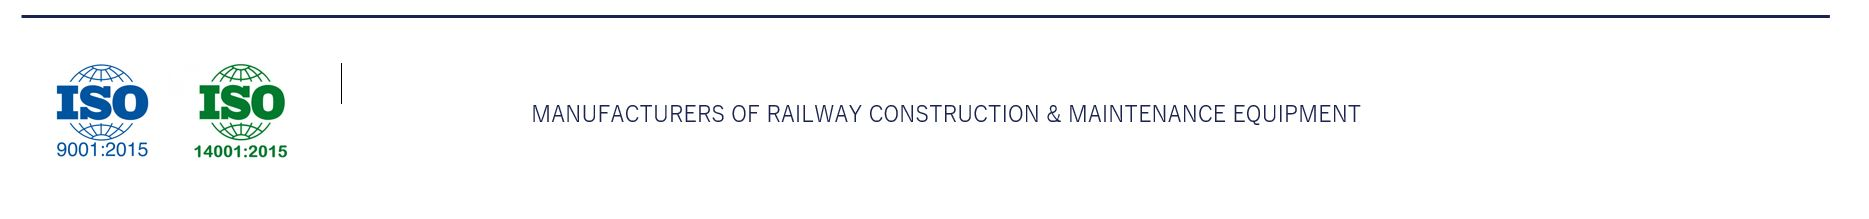
\includegraphics[height=2.3cm]{logo-1.JPG}}}}{}
  }
}{}

\title{\textbf{Hydraulic Speed Calculation Report}}
\author{
\textbf{Doc-No.: {{ doc_no | default('---') }}}\\
Made By: {{ made_by | default('---') }}\\
Checked By: {{ checked_by | default('---') }}\\
Approved By: {{ approved_by | default('---') }}
}
\date{{ doc_date | default("\\today") }}

\begin{document}
\maketitle

%------------------------------------------------
\section*{Input Parameters}

\subsection*{Vehicle Inputs}
\begin{itemize}
  \item Vehicle Weight: {{ weight | default('---') }} t
  \item Total Axles: {{ axles | default('---') }}
  \item Drive Axles: {{ drive_axles | default('---') }}
  \item Wheel Diameter: {{ wheel_diameter | default('---') }} mm
  \item Slope: {{ slope_percent | default(0) }} \%
  \item Curve: {{ curve_degree | default(0) }} deg
  \item Axle Gear Box Ratio: {{ axle_gear_box_ratio | default('---') }}
  \item Engine Gear Ratio(s): {{ engine_gear_ratio_list | default('---') }}
  \item Max Vehicle RPM: {{ max_vehicle_rpm | default('---') }} RPM
\end{itemize}

\subsection*{Hydraulic Inputs}
\begin{itemize}
  \item PTO Gear Ratio: {{ pto_gear_ratio | default('---') }}
  \item Number of Pumps: {{ num_pumps | default('---') }}
  \item Pump Displacement: {{ pump_disp_in | default('---') }} cc/rev
  \item Pump Volumetric Efficiency: {{ vol_eff_pump | default('---') }} \%
  \item Motor Displacement: {{ motor_disp_in | default('---') }} cc/rev
  \item Motor Mechanical Efficiency: {{ mech_eff_motor | default('---') }} \%
  \item System Pressure: {{ pressure | default('---') }} bar
  \item Motors per Axle: {{ per_axle_motor | default('---') }}
  \item Number of Motors: {{ num_motors | default('---') }}
\end{itemize}

%------------------------------------------------
\section*{Gear-wise Hydraulic Calculations}

{% for g in gear_results %}
\subsection*{Gear Ratio = {{ g.gear_ratio | round(2) }}}

\textbf{Step 1: Pump Speed}
\[ Pump\_Speed = \frac{Max\_RPM}{Gear\_Ratio} \times \frac{PTO\_Ratio}{Num\_Pumps} \]
\[ = \frac{ {{ max_vehicle_rpm | default(0) }} }{ {{ g.gear_ratio | round(2) }} } \times \frac{ {{ pto_gear_ratio | default(1) }} }{ {{ num_pumps | default(1) }} } = {{ g.pump_speed | round(2) }} \; RPM \]

\textbf{Step 2: Per Pump Flow}
\[ Q_{pump} = \frac{Pump_{cc} \times Pump\_Speed \times \eta_{vol}}{1000} \]
\[ = \frac{ {{ pump_disp_in | default(0) }} \times {{ g.pump_speed | round(2) }} \times {{ (vol_eff_pump / 100) | round(2) }} }{1000} = {{ g.per_pump_flow | round(2) }} \; LPM \]

\textbf{Step 3: Per Motor Flow}
\[ Q_{motor} = \frac{Q_{pump}}{Drive\_Axles \times Motors\_per\_Axle} \]
\[ = \frac{ {{ g.per_pump_flow | round(2) }} }{ {{ drive_axles | default(1) }} \times {{ per_axle_motor | default(1) }} } = {{ g.per_motor_flow | round(2) }} \; LPM \]

\textbf{Step 4: Available Motor Torque}
\[ T_{avail} = \eta_{mech} \times Pressure \times Motor_{cc} \times 0.015915 \]
\[ = {{ (mech_eff_motor / 100) | round(2) }} \times {{ pressure | default(0) }} \times {{ motor_disp_in | default(0) }} \times 0.015915 = {{ g.avail_torque | round(2) }} \; Nm \]

{% endfor %}

%------------------------------------------------
{% if matched_speed_kph %}
\section*{Resistance \& Torque at Matched Speed}
\subsection*{Matched Condition: {{ matched_speed_kph }} km/h @ Gear Ratio {{ matched_gear_ratio | round(2) }}}

\textbf{Step 1: Resistance Coefficients}
\[ A = 0.647 + \frac{13.17}{W / Axles} = 0.647 + \frac{13.17}{ {{ weight | default(0) }} / {{ axles | default(1) }} } = {{ coeff_A | default(0) | round(2) }} \]
\[ B = 0.00933 \]
\[ C = \frac{0.057}{W} = \frac{0.057}{ {{ weight | default(0) }} } = {{ coeff_C | default(0) | round(2) }} \]

\textbf{Step 2: Resistance Forces at V = {{ matched_speed_kph }} km/h}
\[ F_{rolling} = (A + B \cdot V + C \cdot V^2) \times W \times g / 1000 \]
\[ = ( {{ coeff_A | default(0) | round(2) }} + {{ coeff_B | default(0) }} \times {{ matched_speed_kph }} + {{ coeff_C | default(0) | round(2) }} \times {{ matched_speed_kph }}^2 ) \times {{ weight | default(0) }} \times 9.81 / 1000 = {{ rolling_resistance | default(0) | round(2) }} \; kN \]

\[ F_{gradient} = \frac{W \times 1000 \times g \times slope}{100000} = \frac{ {{ weight | default(0) }} \times 1000 \times 9.81 \times {{ slope_percent | default(0) }} }{100000} = {{ gradient_resistance | default(0) | round(2) }} \; kN \]

\[ F_{curve} = \frac{0.4 \times W \times curve \times g}{1000} = \frac{0.4 \times {{ weight | default(0) }} \times {{ curve_degree | default(0) }} \times 9.81}{1000} = {{ curvature_resistance | default(0) | round(2) }} \; kN \]

\[ F_{starting} = \frac{6 \times W \times g}{1000} = \frac{6 \times {{ weight | default(0) }} \times 9.81}{1000} = {{ starting_resistance | default(0) | round(2) }} \; kN \]

\[ F_{total} = {{ rolling_resistance | default(0) | round(2) }} + {{ gradient_resistance | default(0) | round(2) }} + {{ curvature_resistance | default(0) | round(2) }} + {{ starting_resistance | default(0) | round(2) }} = {{ total_resistance | default(0) | round(2) }} \; kN \]

\textbf{Step 3: Torque Requirement}
\[ r = \frac{wheel\_dia}{2000} = \frac{ {{ wheel_diameter | default(0) }} }{2000} = {{ wheel_radius | default(0) | round(2) }} \; m \]

\[ T_{total} = F_{total} \times 1000 \times r = {{ total_resistance | default(0) | round(2) }} \times 1000 \times {{ wheel_radius | default(0) | round(2) }} = {{ required_total_torque | default(0) | round(2) }} \; Nm \]

\[ T_{per\,axle} = \frac{T_{total}}{Drive\_Axles} = \frac{ {{ required_total_torque | default(0) | round(2) }} }{ {{ drive_axles | default(1) }} } = {{ per_axle_torque | default(0) | round(2) }} \; Nm \]

\[ T_{per\,motor\,(req)} = \frac{T_{per\,axle}}{Motors\_per\_Axle \times Axle\_Gear\_Ratio} = \frac{ {{ per_axle_torque | default(0) | round(2) }} }{ {{ per_axle_motor | default(1) }} \times {{ axle_gear_box_ratio | default(1) }} } = {{ per_gearbox_input_torque | default(0) | round(2) }} \; Nm \]

\textbf{Step 4: Torque Match Check}
\[ T_{avail} = {{ available_torque | default(0) | round(2) }} \; Nm \geq T_{req} = {{ per_gearbox_input_torque | default(0) | round(2) }} \; Nm \quad \checkmark \]
\begin{center}
\textbf{\large Matched Speed = {{ matched_speed_kph }} km/h @ Gear Ratio {{ matched_gear_ratio | round(2) }}}
\end{center}

{% else %}
\section*{No Achievable Speed Found}

\[ T_{avail} = {{ available_torque | default(0) | round(2) }} \; Nm < T_{req\,(min)} = {{ min_required_torque | default(0) | round(2) }} \; Nm \]

\begin{center}
\textbf{At the given slope ({{ slope_percent | default(0) }}\%), curve ({{ curve_degree | default(0) }} deg) and gear ratio(s) {{ engine_gear_ratio_list | default('---') }}, the available motor torque is insufficient to move the vehicle at any speed.}
\end{center}

\textbf{Suggestions to achieve a match:}
\begin{itemize}
  \item Increase system pressure (currently {{ pressure | default(0) }} bar)
  \item Increase motor displacement (currently {{ motor_disp_in | default(0) }} cc/rev)
  \item Reduce slope or vehicle weight
\end{itemize}
{% endif %}

\end{document}
